% !TeX spellcheck = en_GB
\documentclass[10pt,letterpaper,oneside]{article}
\usepackage{fontspec}
\usepackage{arev}
\usepackage[utf8]{inputenc}
\usepackage[T1]{fontenc}
\usepackage{amsmath}
\usepackage{amsfonts}
\usepackage{amssymb}
\usepackage{graphicx}
\usepackage{csquotes}
\usepackage{booktabs}
\usepackage{multicol}
\usepackage{enumerate}
\usepackage{microtype}
\usepackage[labelfont=bf,font={small}]{caption}
\usepackage{hyperref}
\usepackage{booktabs}
\usepackage{subcaption}
\usepackage{fancyhdr}
\usepackage[svgnames]{xcolor}
\usepackage{mdframed}
\usepackage{multicol}
\usepackage[para]{footmisc}
\usepackage{siunitx}
\usepackage{cleveref}
\usepackage{listings}
\usepackage{cprotect}


\lstset{ % General setup for the package
	language=Python,
	basicstyle=\small\ttfamily,
	tabsize=4,
	columns=fixed,
	showstringspaces=false,
	showtabs=false,
	keepspaces,
	commentstyle=\color{SeaGreen},
	keywordstyle=\bf\ttfamily\color{DarkBlue}
}

\newfontfamily\symbolfont{Symbola}
\usepackage[left=1in,right=1in,top=1in,bottom=1in,marginparwidth=0.3in]{geometry}

\usepackage[sorting=none]{biblatex}
\addbibresource{../bibliography.bib}

\author{Andreas Stöckel\\[0.5cm]Based on lecture notes by\\Chris Eliasmith and Terrence~C.~Stewart}
\newcommand{\baseCodeURL}{https://github.com/astoeckel/syde556-w20/blob/master/lectures}

\fancyhf{}
\fancyhead[L]{SYDE 556/750 Lecture Notes}
\fancyhead[R]{Andreas Stöckel}
\fancyfoot[C]{\thepage}
\pagestyle{fancy}

\setlength{\parindent}{0em}
\setlength{\parskip}{0.5em}
\renewcommand{\baselinestretch}{1.25}
\renewcommand{\vec}[1]{{\mathbf{#1}}}
\newcommand{\mat}[1]{{\mathbf{#1}}}
\newcommand{\T}{\ensuremath{\mathrm{T}}}
\renewcommand{\epsilon}{\varepsilon}
\renewcommand{\phi}{\varphi}

\makeatletter
\newcommand{\superimpose}[2]{%
	{\ooalign{{#1}\hidewidth\cr{#2}\hidewidth\cr}}}
\makeatother
\newcommand{\SolidCircle}[2]{\superimpose{\color{#1}\symbolfont ⬤}{\textbf{\color{white}#2}}\hspace{1em}}
\newcommand{\OPlus}{\SolidCircle{DarkGreen}{\kern0.75pt+}}
\newcommand{\OMeh}{\SolidCircle{DarkOrange}{~}}
\newcommand{\OMinus}{\SolidCircle{DarkRed}{\kern2.25pt--}}

\newcommand{\YouTube}[2][Video]{\href{https://youtu.be/#2}{{\symbolfont 📺}~{#1}}%
%\footnote{\url{https://youtu.be/#2}}%
}

\newcommand{\CodeLink}[2][Code]{\href{\baseCodeURL/#2}{{\symbolfont ⌨}~\emph{#1}}}

\newcommand{\MakeTitle}[1]{
\maketitle
\begin{center}
	
\includegraphics[width=0.5\textwidth]{../assets/uwlogo.pdf}\\[1cm]
	{#1}\
\end{center}

\vfill

\thispagestyle{empty}
\setcounter{page}{0}
\newpage

\pagenumbering{roman}
\setcounter{tocdepth}{2}
\tableofcontents
\newpage

\setcounter{page}{0}
\pagenumbering{arabic}}

\reversemarginpar


\newcommand{\ColorBox}[3]{%
	\marginpar{%
		\huge\raisebox{-3ex}{\symbolfont{#1}}%
	}%
	\begin{mdframed}[hidealllines=true,backgroundcolor=#2,innertopmargin=0.25cm,innerbottommargin=0.25cm]%
		{#3}
	\end{mdframed}}

\newcommand{\Note}[1]{\ColorBox{📌}{WhiteSmoke}{\textbf{Note:} #1}}
\newcommand{\Example}[1]{\ColorBox{💡}{WhiteSmoke}{\textbf{Example:} #1}}
\newcommand{\Aside}[1]{\ColorBox{🌟}{WhiteSmoke}{\emph{Aside:} #1}}
\newcommand{\Python}[1]{\ColorBox{🐍}{WhiteSmoke}{#1}}
\newcommand{\Notation}[1]{\ColorBox{\huge$\Sigma$}{WhiteSmoke}{\textbf{Notaton:} #1}}

\newcommand{\ConstructionSite}{\hrulefill {\symbolfont 🚧} UNDER CONSTRUCTION {\symbolfont 🚧} \hrulefill}

\newenvironment{ImportantEqn}[1]{\mdframed\raggedleft\emph{({#1})}\align}{\endalign\endmdframed}

\date{March 10 \& 12, 2020}
\title{SYDE 556/750 \\ Simulating Neurobiological Systems \\ Lecture 10: Symbols and Symbol-like Representations}


\begin{document}

\MakeTitle{\textbf{Accompanying Readings: Chapter 3, 4 and 9 of \enquote{How to Build a Brain}}}

\section{Introduction}

\Note{So far we have mostly been concerned with representing vectors $\vec x$ in populations of neurons. In this lecture we instead think about the representation of \emph{symbols}, leading up to the Semantic Pointer Architecture (SPA).}

As discussed at the beginning of the lecture, our ultimate goal is to build models of human brains, and, by extension, human cognition. So far it seems as if had not made much progress in this direction. What we have discussed so far is \enquote{merely} allowing us to represent vectors in a population of neurons, to compute transformations of the represented values within the connections between populations, and to build dynamical systems treating the represented values as control-theoretic state variables.

In particular, one hallmark of human cognition is \emph{language}. So far, it is not clear how to apply the NEF to language, or facts expressed in language, such as \enquote{the number eight comes after the number nine}, \enquote{all dogs chase cats}, \enquote{Anne knows that Bill thinks that Charlie likes Dave}.

We attempt to solve this problem by first having a look at other modelling approaches in Cognitive Science. In particular, we will have a look at so called Vector Symbolic Architectures (VSAs), which can be easily mapped onto the NEF. We then use VSAs to build a particular model of cognition, the Semantic Pointer Architecture (SPA).

\section{Neural Theories of Cognition}

\Note{For more details on theories of cognition, have a look at Chapter 9 of \enquote{How to Build a Brain}~\cite{eliasmith2013how}.}

Traditionally, cognitive scientists (and computer scientists) have been working on theories of cognition that involve structured information using some kind of representational framework, such as predicate logic. For example, the first two facts mentioned above could be written in predicate logic like this:
\newcommand{\Pred}[1]{\mathbf{\textcolor{Crimson}{#1}}}
\newcommand{\Obj}[1]{\mathtt{\textcolor{RoyalBlue}{#1}}}
\newcommand{\Fun}[1]{\mathit{\textcolor{ForestGreen}{#1}}}
\begin{itemize}
	\item \enquote{The number eight comes after the number nine}: $\Pred{isSucc}(\Obj{EIGHT}, \Obj{NINE})\,$.
	\item \enquote{All dogs chase cats}: $\forall x \forall y \, \big ( \Pred{isDog}(x) \wedge \Pred{isCat}(y) \big) \rightarrow \Pred{doesChase}(x, y)\,$.
	\item \enquote{Anne knows that Bill thinks that Charlie likes Dave}:$$\Pred{knows}\Big(\Obj{ANNE}, ``\Pred{thinks}\big(\Obj{BILL}, `\Pred{likes}(\Obj{CHARLIE}, \Obj{DAVE})\text{'}\big)\text{''}\Big)\,.$$
\end{itemize}
Both computer scientists and cognitive scientists have successfully built cognitive models which are roughly based on representations akin to the ones listed above. These \enquote{symbolic} approaches are generally quite successful in modelling aspects of human cognition and can match behavioural data. However, they do not answer the question of how these symbols are represented and manipulated within a human brain.

\subsection{Jackendoff's Challenges for Cognitive Neuroscience}

In his 2002 book \enquote{Foundations of Language: Brain, Meaning, Grammar, Evolution} \cite{jackendoff2002foundations}, linguist Ray Jackendoff poses four challenges cognitive neuroscientists who aim to build a neural model of language. These challenges are
\newcommand{\RS}{$\color{Crimson}\blacksquare$}
\newcommand{\BC}{$\color{RoyalBlue}\bullet$}
\begin{itemize}
	\item \textbf{The Binding Problem.} Suppose you see a red square and a blue circle. Now, how does the concept of \enquote{red} get bound with the concept of \enquote{square}, and how is it kept separate from \enquote{blue} and \enquote{circle}?
	\item \textbf{The Problem of Two.} Consider the sentence \enquote{the little star is besides the big star}. How do we keep those two uses of the concept \enquote{star} separate? For example, if there was group of neurons representing the concept of \enquote{star}, how can this group of neurons both represent the \enquote{little star}, the \enquote{large star}, as well as the fact that the two stars are next to each other.
	\item \textbf{The Problem of Variables.} Grammar imposes certain rules on sentences. For example, it is \enquote{correct} to say \enquote{blue $x$}, if $x$ is a noun, but not \enquote{blue $y$}, if $y$ is a verb. Correspondingly, the question is how these rules, which rely on placeholders, or \enquote{variables}, are represented in the brain.
	\item \textbf{Working Memory versus Long-Term Memory.} We can both \emph{use} sentences (working memory; i.e., current neural activities), while also being able to \emph{store} them for very long times (long-term memory; synaptic weights). A neural architecture of language must explain how sentences can be transferred from working memory to long-term memory and back. In other words, we must be able to turn representations from neural activities into synaptic weight changes.
\end{itemize}

\subsection{Solution Attempt 1: Neural Synchrony (Oscillations)}

\begin{figure}
	\centering
	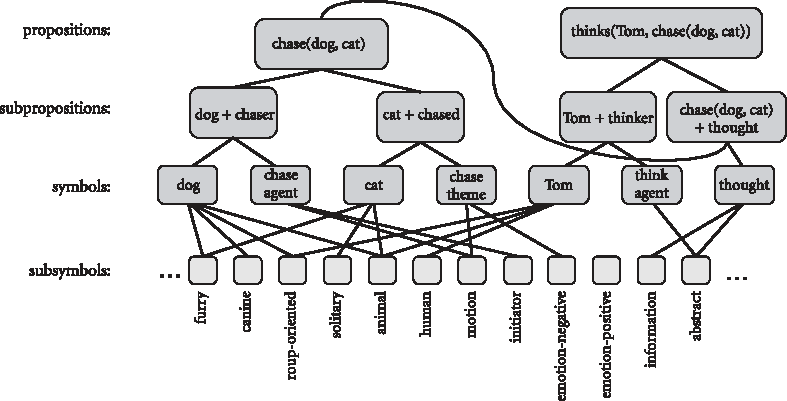
\includegraphics[width=\textwidth]{media/eliasmith_2013_lisa.pdf}
	\caption{The LISA architecture. Boxes corresponds to groups of neurons representing individual concepts, lines to synaptic conncetions. Concepts are \enquote{bound} together by neurons oscillating at the same frequency. Figure copied from Figure~9.1~in Eliasmith, 2013 \cite{eliasmith2013how}, which is in turn adapted from Hummel and Holyoak, 2003~\cite{hummel2003symbolicconnectionist}.}
	\label{fig:eliasmith_2013_lisa.pdf}
\end{figure}

One of the earliest theories of how the \enquote{binding problem} could be solved is the LISA architecture \cite{hummel2003symbolicconnectionist}, which has been developed in the early 1990s. This architecture solves the binding problem by proposing to exploit what is known as neural synchrony.

A central idea of this approach is that individual groups of neurons represent concepts---this is a so called \emph{localist} representation; individual spatially colocated groups of neurons correspond to individual concepts. Higher-level concepts can be created by connecting groups of neurons. For example, the neurons representing the symbol \enquote{cat} can be connected to neurons representing the concepts \enquote{furry}, \enquote{solitary}, and \enquote{animal} (cf.~\cref{fig:eliasmith_2013_lisa.pdf}).

Concepts are bound together by neurons representing the concept oscillating at the same frequency. That is, for our example of \enquote{red square and blue circle}, the neuron populations of these concepts would oscillate synchronously in phase, while separate, currently active concepts oscillate with a different frequency and/or out of phase.

\newpage

Let's evaluate this architecture.
\begin{itemize}
	\item[\OPlus] The architecture solves the binding problem.
	\item[\OMeh] The architecture assumes localist representation, i.e., a few neurons represent a single concept. Most evidence points towards a distributed representation.
	\item[\OMeh] It is unclear how this architecture would solve the \enquote{problem of two} -- maybe the same symbol used multiple times could oscillate with two superimposed frequencies.
	\item[\OMeh] This architecture cannot solve Jackendoff's third and fourth challenge.
	\item[\OMinus] It is unclear how these oscillations are generated and controlled in the first place, i.e., how is language translated into activation of these localist representations?
	\item[\OMinus] Furthermore, it us unclear how the representations are processed---which mechanism is reading out the oscillations and decides which neural ensembles are active together?
	\item[\OMinus] Finally, we have an exponential explosion of neurons required to represent all kinds of different concepts. For example, assume that there are $10^4$ symbols. Then, we have on the order of $10^8$ possible second-order combinations of symbols (\enquote{subpropositions}), and on the order of $10^{16}$ possible propositions. This already exceeds the number of neurons in the brain by a factor of one to ten thousand.
\end{itemize}

\subsection{Solution Attempt 2: Neural Blackboard Architecture}

\begin{figure}[t]
	\centering
	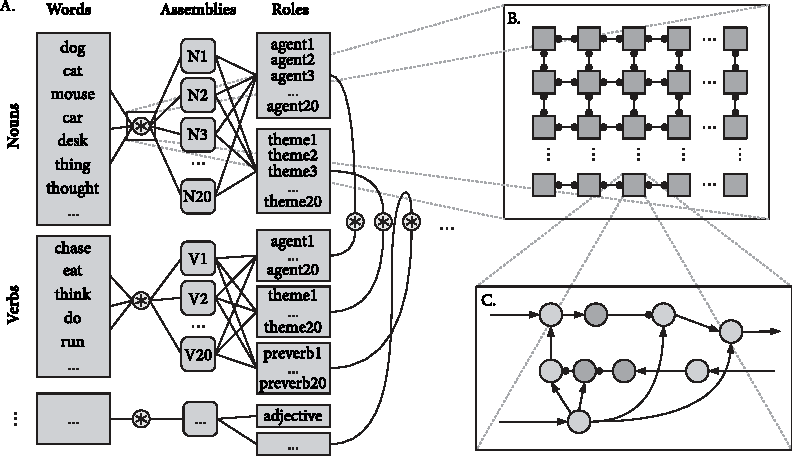
\includegraphics[width=\textwidth]{media/eliasmith_2013_blackboard.pdf}
	\caption{Neural Blackboard Architecture. \textbf{(a)} Groups of neurons represent concepts (words)---they are connected via a switchboard circuit (symbolised by $\circledast$ and depicted in panels \textbf{(b)} and \textbf{(c)}) to slots corresponding to individual roles in a sentence. These roles are then combined via switchboards into higher-level sentences. Image copied from Figure~9.2~in Eliasmith, 2013~\cite{eliasmith2013how}, which is in term adapted from van der Velde and de Kamps, 2006~\cite{vandervelde2006neural}.}
\end{figure}

An attempt at solving all four problems posed by Jackendoff is the \enquote{Neural Blackboard Architecture} by van der Velde and de Kamps~\cite{vandervelde2006neural}, solving the exponential growth problem posed by synchrony approaches. In particular, the idea is to introduce switchboard circuits that can arbitrarily route signals from neurons representing individual concepts to assemblies (a \enquote{temporary pool}) representing bound concepts. These high level concepts can then be associated with specific roles a concept might have in a sentence.
\begin{itemize}
	\item[\OPlus] This approach has a much lower resource consumption than LISA.
	\item[\OPlus] Can solve all four of Jackendoffs challenges (according to the authors).
	\item[\OPlus] Explains limitations of human sentence representation.
	\item[\OMeh] This is still a (at least partially) localist representation.
	\item[\OMinus] Uses a very particular structure that does not really seem to match biology.
	\item[\OMinus] Uses a very large number of neurons; about $500\times 10^6$ to represent simple sentences.
	\item[\OMinus] Only considers sentence representation, but not the individual control structures.
\end{itemize}

\subsection{Solution Attempt 3: Vector Operators}

As mentioned, both approaches discussed above are \emph{localist}. We could instead decouple concepts from the underlying neural substrate. That is, populations of neurons can represent different symbols, and send represented symbols for processing to other groups of neurons.

This would be more in line with what the NEF suggests, and knowing that we can represent vectors in neural populations, we could thus represent symbols by assigning vectors $\vec x \in \mathbb{R}^d$ to individual symbols. For now, we assume that these vectors $\vec x$ have been randomly generated.

This idea is actually quite old, and there have been multiple suggestions as for how to symbol vectors $\vec x$ and $\vec y$ could be bound together. One approach suggested by Smolensky in 1990 \cite{smolensky1990tensor} is to simply use a tensor product $\vec x \otimes \vec y$, a generalisation of a vector outer product to matrices:
\begin{align*}
	\begin{pmatrix}a_1\\a_2\\a_3\end{pmatrix} \otimes \begin{pmatrix}b_1\\b_2\\b_3\end{pmatrix} &=
	\begin{pmatrix}
		a_1 b_1 & a_1 b_2 & a_1 b_3 \\
		a_2 b_1 & a_2 b_2 & a_2 b_3 \\
		a_3 b_1 & a_3 b_2 & a_3 b_3
	\end{pmatrix} && \text{(Outer product)} \\
	\begin{pmatrix}a_{11} & a_{12} \\ a_{21} & a_{22} \end{pmatrix} \otimes
	\begin{pmatrix}b_{11} & b_{12} \\ b_{21} & b_{22} \end{pmatrix} &=
	\begin{pmatrix}
		a_{11} \begin{pmatrix}b_{11} & b_{12} \\ b_{21} & b_{22} \end{pmatrix} &
		a_{12} \begin{pmatrix}b_{11} & b_{12} \\ b_{21} & b_{22} \end{pmatrix} \\
		a_{21} \begin{pmatrix}b_{11} & b_{12} \\ b_{21} & b_{22} \end{pmatrix} &
		a_{22} \begin{pmatrix}b_{11} & b_{12} \\ b_{21} & b_{22} \end{pmatrix}
	\end{pmatrix} && \text{(Tensor product)}\\ &= 
	\begin{pmatrix}
		a_{11} b_{11} & a_{11} b_{12} & a_{12} b_{11} & a_{12} b_{12} \\
		a_{11} b_{21} & a_{11} b_{22} & a_{12} b_{21} & a_{12} b_{22} \\
		a_{21} b_{11} & a_{21} b_{12} & a_{22} b_{11} & a_{22} b_{12} \\
		a_{21} b_{21} & a_{21} b_{22} & a_{22} b_{21} & a_{22} b_{22}
	\end{pmatrix}
\end{align*}
This way, two vectors $\vec x$, $\vec y$ can be bound without losing any information. In contrast to just stacking the two vectors (which would also not incur any information loss), the tensor product has some nice mathematical properties, and can, as outlined by Smolensky in his paper, to a degree be easily implemented in a neural substrate.
\begin{itemize}
	\item[\OPlus] Solves the binding problem and the problem of two.
	\item[\OMeh] Unclear how to solve Jackendoff's third and fourth challenge.
	\item[\OMinus] The method scales extremely poorly. Every time two vectors are bound, the dimensionality of the resulting structure is squared; we need $d^2$ dimensions when binding two $d$-dimensional vectors. In general, for $n$ binding operations we need $d^n$ dimensions.
\end{itemize}

\Note{\emph{Symbolic Architectures and Neuroscience.} All methods discussed so far are trying very hard to map purely symbolic architectures onto a neural substrate. In a sense, neural aspects are treated as \emph{mere implementation details}. This is an instance of the top-down approach we discussed at beginning of the course: mapping high-level cognitive architectures onto biology. In a sense, the hope is that, if successful, neurons would not matter. This is (unfortunately) an assumption many cognitive scientists make.}

\section{Vector Symbolic Architectures}

The last idea---using vectors $\vec x$ to represent symbols and to then use an operator such as $\otimes$ to bind them---seems to be reasonable, and fits the Neural Engineering Framework quite well. However, what we would like to have is an operator that maintains the size of the vectors (i.e., takes two vectors of dimensionality $d$ as an input and outputs a vector of dimensionality $d$), while still allowing us to reconstruct information about the operands.

\Example{\emph{Using \enquote{$+$} as a binding operator}.
Let's reconsider the \enquote{Binding Problem} as originally posed above. We would like to represent the fact that we are seeing a blue square and a red circle. Hence, we could---for now, randomly---generate four $d$-dimensional vector representing these four concepts, where $d$ is relatively large, for example $d = 64$. 

To keep us from having to come up with letters $\vec x$, $\vec y$, $\vec z$, $\vec w$, \textellipsis for each concept and remember the mapping between letter and concept, we will just write the vector corresponding to each concept in capital letters, like so: $\Obj{BLUE}$, $\Obj{RED}$, $\Obj{CIRCLE}$, $\Obj{SQUARE}$. Keep in mind that this is just notation; each of these words is a (random), $d$-dimensional vector.

Our first attempt at representing the above concept could be to just sum these vectors
\begin{align*}
	\vec x = \Obj{BLUE} + \Obj{SQUARE} + \Obj{RED} + \Obj{CIRCLE} \,.
\end{align*}
However, notice that mere addition of symbol vectors does not allow us to distinguish which colour belongs to which object. Correspondingly, \enquote{$+$} is not a good choice as a binding operator, but may be used to represent that two separate concepts are currently active.}

\newcommand{\CC}{\circledast}
Mathematically, what we would like is an operator $\CC$ with the following properties
\begin{align*}
	\CC &: \mathbb{R}^d \times \mathbb{R}^d \longrightarrow \mathbb{R}^d \,, && \text{(preservation of dimensionality)} \\
	\vec x &\approx (\vec x \CC \vec y) \CC \vec y^{-1} \,, && \text{(approximately reversible)} \\
	0 &\approx \langle \vec x \CC \vec y, \vec x \rangle \,, 0 \approx \langle \vec x \CC \vec y, \vec y \rangle \,. && \text{(dissimilar to inputs)}
\end{align*}
As we have discussed in the above example, the last property ensures that two concepts that are bound to each other cannot be confused with the original concepts. This prevents us from using an operator such as \enquote{$+$} as a binding operator, which preserves similarity, as graphically depicted in \cref{fig:cconv_sim}, and as can be easily shown:
\begin{align*}
	\langle \vec x + \vec y, \vec x \rangle = \langle \vec x, \vec x \rangle + \langle \vec x, \vec y \rangle \approx \|\vec x\|^2 + 0 \,,
\end{align*}
assuming that $\vec x$ and $\vec y$ are two high-dimensional random vectors, which are likely to be orthogonal. We will still use \enquote{$+$} to combine multiple concepts into one symbolic vector.

The use of (random) vectors $\vec x$ along with a binding operator $\otimes$ to construct cognitive symbolic architectures have been called \enquote{Vector Symbolic Architectures} (VSAs) by Gayler, 2003 \cite{gayler2003vector}. In the same paper, Gayler argues that such architectures can solve all four challenges put forward by Jackendoff.

\begin{figure}
	\centering
	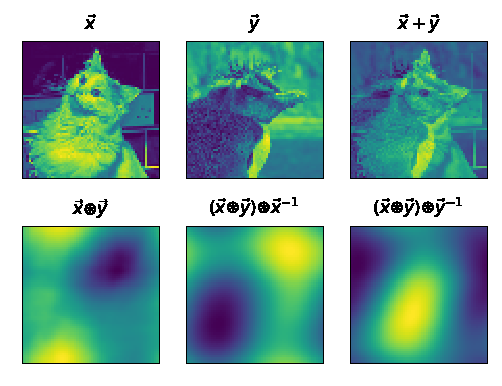
\includegraphics{media/cconv_sim.pdf}
	\caption{Similarity preservation and approximate reversibility of circular convolution. The $+$ operator preserves similarity between $\vec x$, $\vec y$ (both the penguin and the cat are still visible), whereas circular convolution $\circledast$ does not (neither the penguin nor the cat are visible). Convolving $\vec x \circledast \vec y$ with the pseudo-inverse $\vec x^{-1}$ and $\vec y^{-1}$ creates an image that is more similar to $\vec y$ and $\vec x$, respectively. The use of images in this example does not imply that we usually apply these methods to uncompressed images. \CodeLink{lecture_10/media/code/cconv_similarity.ipynb}}
	\label{fig:cconv_sim}
\end{figure}

\newpage
\Example{\emph{Possible Binding Operators.} Among others, the following binding operators have been proposed for use in vector symbolic architectures:
\begin{align*}
	\begin{pmatrix}1 \\ 0 \\ 1 \\ 0\end{pmatrix} \oplus \begin{pmatrix}1 \\ 1 \\ 0 \\ 0\end{pmatrix} &= \begin{pmatrix}0 \\ 1 \\ 1 \\ 0\end{pmatrix} && \textit{(XOR)}\\
	\begin{pmatrix}A \\ B \\ C \\ D\end{pmatrix} \odot \begin{pmatrix}E \\ F \\ G \\ H\end{pmatrix} &= \begin{pmatrix}AE \\ BF \\ CG \\ DH\end{pmatrix} && \textit{(Hadamard Product)} \\
	\begin{pmatrix}A \\ B \\ C \\ D\end{pmatrix} \CC \begin{pmatrix}E \\ F \\ G \\ H\end{pmatrix} &= \begin{pmatrix}AE &+& BH &+& CG &+& DF \\ AF &+& BE &+& CH &+& DG \\ AG &+& BF &+& CE &+& DH \\ AH &+& BG &+& CF &+& DE\end{pmatrix} && \textit{(Circular Convolution)}
\end{align*}
Circular convolution compresses the outer product by summation along the diagonals:\\[0.25cm]
\hspace*{1.315cm}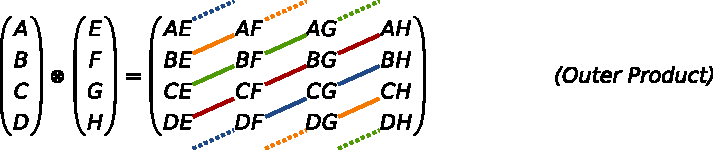
\includegraphics{media/cconv_outer_product.pdf}
%\begin{align*}
%	\begin{pmatrix}A \\ B \\ C \\ D\end{pmatrix} \otimes \begin{pmatrix}E \\ F \\ G \\ H\end{pmatrix} &=
%	\begin{pmatrix}AE & \vphantom{+} & AF & \vphantom{+} & AG & \vphantom{+} & AH\\
%	               BE & \vphantom{+} & BF & \vphantom{+} & BG & \vphantom{+} & BH\\
%                   CE & \vphantom{+} & CF & \vphantom{+} & CG & \vphantom{+} & CH\\
%                   DE & \vphantom{+} & DF & \vphantom{+} & DG & \vphantom{+} & DH\end{pmatrix} && \textit{(Outer Product)}
%\end{align*}
}


\subsection{Examples: Binding and Unbinding}
We can use the binding operator \enquote{$\circledast$} and the plus operator \enquote{$+$} to encode all kinds of information in a single vector. For example, we can now write the above example as
\begin{align*}
	\vec x = \Obj{BLUE} \CC \Obj{SQUARE} + \Obj{RED} \CC \Obj{CIRCLE} \,.
\end{align*}
We can use the reversibility property to \enquote{ask questions}. For example, \enquote{which object is blue?}
\begin{align*}
	\vec y &= \big( \Obj{BLUE} \CC \Obj{SQUARE} + \Obj{RED} \CC \Obj{CIRCLE} \big) \CC \Obj{BLUE}^{-1} \\
		   &= \big( \Obj{BLUE} \CC \Obj{SQUARE} \big) \CC \Obj{BLUE}^{-1} + \big( \Obj{RED} \CC \Obj{CIRCLE} \big) \CC \Obj{BLUE}^{-1} \\
		   &\approx \Obj{SQUARE} + 0 \,.
\end{align*}

We can use this technique to write down more interesting concepts, such as the sentences we talked about in the previous section:
\begin{itemize}
	\item \enquote{The number eight comes after the number nine}:
	\begin{align*}
		\Obj{NUMBER} \CC \Obj{EIGHT} + \Obj{SUCC} \CC \Obj{NINE} \,.
	\end{align*}
	\item \enquote{The dog chases the cat}:
	\begin{align*}
		\Obj{DOG} \CC \Obj{SUBJ} + \Obj{CAT} \CC \Obj{OBJ} + \Obj{CHASE} \CC \Obj{VERB} \,.
	\end{align*}
	\item \enquote{Anne knows that Bill thinks that Charlie likes Dave}:
	\begin{align*}
	 	\Obj{SUBJ} \CC \Obj{ANNE} + \Obj{ACT} \CC \Obj{KNOWS} + \Obj{OBJ} \CC \\\Big(\Obj{SUBJ} \CC \Obj{BILL} + \Obj{ACT} \CC \Obj{THINKS} + \Obj{OBJ} \CC \\ \big(\Obj{SUBJ} \CC \Obj{CHARLIE} + \Obj{ACT} \CC \Obj{LIKES} + \Obj{OBJ} \CC \Obj{DAVE}\big)\Big) \,.
	\end{align*}
\end{itemize}
\Note{\emph{Graceful degradation.}
The information we can pack into a single vector $\vec x$ is limited! The larger the number of binding operations, and the number of additions, the lower the precision of operations such as the approximate inverse. While this may sound bad, humans have similar limitations: for example, the nesting depth of sentences, or the number of objects we can keep in working memory is limited. This makes for interesting predictions if we use VSAs to model cognitive phenomena.}

\subsection{Circular Convolution}

\begin{itemize}
	\item \enquote{Default convolution operator} to use in conjunction with the NEF
	\item Exhaustively studied by Tony Plate in the 1990s \cite{plate1995holographic}
	\item Has the properties demanded above (see \cref{fig:cconv_sim})
	\item Definition $\vec z = \vec x \CC \vec y$:
	\begin{align*}
		z_i &= \sum_{j = 0}^{d - 1} x_{j} y_{i - j \hspace{-1.25mm} \mod d } \,.
	\end{align*}
	\item Alternatively, can use the DFT:
	\begin{align*}
		\vec z &= \mathcal{DFT}^{-1} \big( \mathcal{DFT}(\vec x) \odot \mathcal{DFT}(\vec y) \big) \\
		       &= \mat T^{-1} \big( \mat T \vec x \odot \mat T \vec y \big)
	\end{align*}
	\item Can be easily implemented in the NEF; three constant linear transformations and a multiplication
\end{itemize}

\subsection{Jackendoff's Challenges}

\begin{itemize}
	\item The Binding Problem: See above
	\item The Problem of Two: Use symbols denoting roles
	\begin{align*}
		\Obj{OBJ1} \CC (\Obj{TYPE} \CC \Obj{STAR} + \Obj{SIZE} \CC \Obj{LITTLE}) + \Obj{OBJ2} \CC (\Obj{TYPE} \CC \Obj{STAR} + \Obj{SIZE} \CC \Obj{BIG}) + \Obj{REL} \CC \Obj{BESIDES}
	\end{align*}
	\item The Problem of Variables: How can we manipulate abstract placeholders?
	\begin{align*}
		 \Obj{S} &= \Obj{RED} \CC \Obj{NOUN}
\\
		 \Obj{VAR} &= \Obj{BALL} \CC \Obj{NOUN}^{-1} \\
		 \Obj{S} \CC \Obj{VAR} &= \Obj{RED} \CC \Obj{BALL}
	\end{align*}
	\item Working vs. Long-Term Memory:
	\begin{itemize}
		\item Working memory: activity of neurons, currently represented concepts $\vec x$
		\item Long term memory: connection weights, functions
		\item Functions can return and modify $\vec x$
	\end{itemize}
\end{itemize}

\section{The Semantic Pointer Architecture}

\begin{itemize}
	\item Combination of multiple ideas:
	\begin{itemize}
		\item NEF
		\item VSAs (with circular convolution; other binding operators possible)
		\item Basal Ganglia/Thalamus/Cortex control loop
		\item Theory as for where $\vec x$ comes from; \emph{compression} and \emph{decompression} $\Rightarrow$ Semantic Pointers
	\end{itemize}
\end{itemize}

\printbibliography

\end{document}

